\documentclass[a4paper, 12pt]{article}
\usepackage[a4paper,top=1.5cm, bottom=1.5cm, left=1cm, right=1cm]{geometry}
\usepackage{cmap}					% поиск в PDF
\usepackage{mathtext} 				% русские буквы в фомулах
\usepackage[T2A]{fontenc}			% кодировка
\usepackage[utf8]{inputenc}			% кодировка исходного текста
\usepackage[english,russian]{babel}	% локализация и переносы

\usepackage{amsmath}
\usepackage{indentfirst}
\usepackage{longtable}
\usepackage{graphicx}
\usepackage{array}

\usepackage{wrapfig}
\usepackage{siunitx} % Required for alignment
\usepackage{subfigure}
\usepackage{multirow}
\usepackage{rotating}
\usepackage{caption}

\graphicspath{{pictures/}}


\title{\begin{center}Лабораторная работа №2.2.6\end{center}
Определение энерги активации по температурной зависимости вязкости жидкости}
\author{Рожков А. В. \\ Руководитель Яворский В. А.}
\date{\today}

\begin{document}
    \pagenumbering{gobble}
    \maketitle
    \newpage
    \pagenumbering{arabic}


    \textbf{Цель работы:} измерение скорости падения шариков при разной температуре жидкости; вычисление вязксоти жидкости по закону Стокса и расчет энергии активации.

    \textbf{В работе используются:} стеклянный цилиндр с исследуемой жидкостью (глицерин); термостат ($\sigma_T = 0.1~К$); секундомер ($\sigma_t = 0.6~сек$); микроскоп ($\sigma_d = 0.02~мм$); мелкие шарики (диаметром 1-2 мм).

    \section{Теоретическая часть}
    \subsection{Энергия активации}
    Для того чтобы перейти в новое состояние, молекула жидкости должна преодолеть участки с большой потенциальной энергией, превышающей среднюю тепловую энергию молекул. Для этого тепловая энергия молекул должна — вследствие флуктуации — увеличиться на некоторую величину $W$ , называемую энергией активации. Температурная зависимость вязкости жидкости при достаточно грубых предположениях можно опистаь формулой
    \begin{equation} \label{activation_energy:1}
        \eta = A e^{W/kT}
    \end{equation}

    Из формулы (\ref{activation_energy:1}) следует, что существует линейня зависимость между величинами $ln\eta$ и $1/T$, и энергию активации можно найти по формуле

    \begin{equation} \label{activation_energy:2}
        W = k \frac{d(ln\eta)}{d(1/T)}
    \end{equation}

    \subsection{Измерение вязкости}
    По формуле Стокса, если шарик радиусом $r$ и со скоростью $v$ движется в среде с вязкостью $\eta$, и при этом не наблюдается турбулентных явлении, тормозящую силу можно найти по формуле (\ref{stokes})

    \begin{equation}\label{stokes}
        F = 6\pi\eta \frac{d}{2}v
    \end{equation}


    Для измерения вязкости жидкости рассмотрим свободное падение шарика в жидкости. При медленных скоростях на шарик действуют силы Архимеда и Стокса, выражения для которых мы знаем. Отсюда находим выражения для установившейся скорости шарика и вязкости жидкости

    \begin{align}
        v_{уст}&=\frac{2}{9}g\frac{d^2}{4}\frac{\rho - \rho_ж}{\eta}\label{v_ust}\\
        \eta&=\frac{2}{9}g\frac{d^2}{4}\frac{\rho - \rho_ж}{v_{уст}}\label{eta}
    \end{align}

    Как видим, измерив установившуюся скорость шарика и параметры системы можно получить вязкость по формуле (\ref{eta}).

    \subsection{Экспериментальная установка}
    Для измерений используется стеклянный цилиндрчиеский сосуд B, наполненный исследуемой жидкостью (глицерин). Диаметр сосуда $\approx 3$ см, длина $\approx 25$ см. На стенках сосуда нанесены две метки на некотором расстоянии друг от друга. Верхняя метка должна располагаться ниже уровня жидкости с таким расчетом, чтобы скорость шарика к моменту прохождения этой метки успевала установиться. Измеряя расстояние между метками, b время падения определяют установившуюся скорость шарика $v_{уст}$. Сам сосуд B помещен в рубашку D, омываемую водой из термостата. При работающем термостате температура воды в рубашке D, а потому и температура жидкости 12 равна температуре воды в термостате.
    Схема прибора (в разрезе) показана на рис.~\ref{ustanovka}.
    \begin{figure}[ht]
        \center{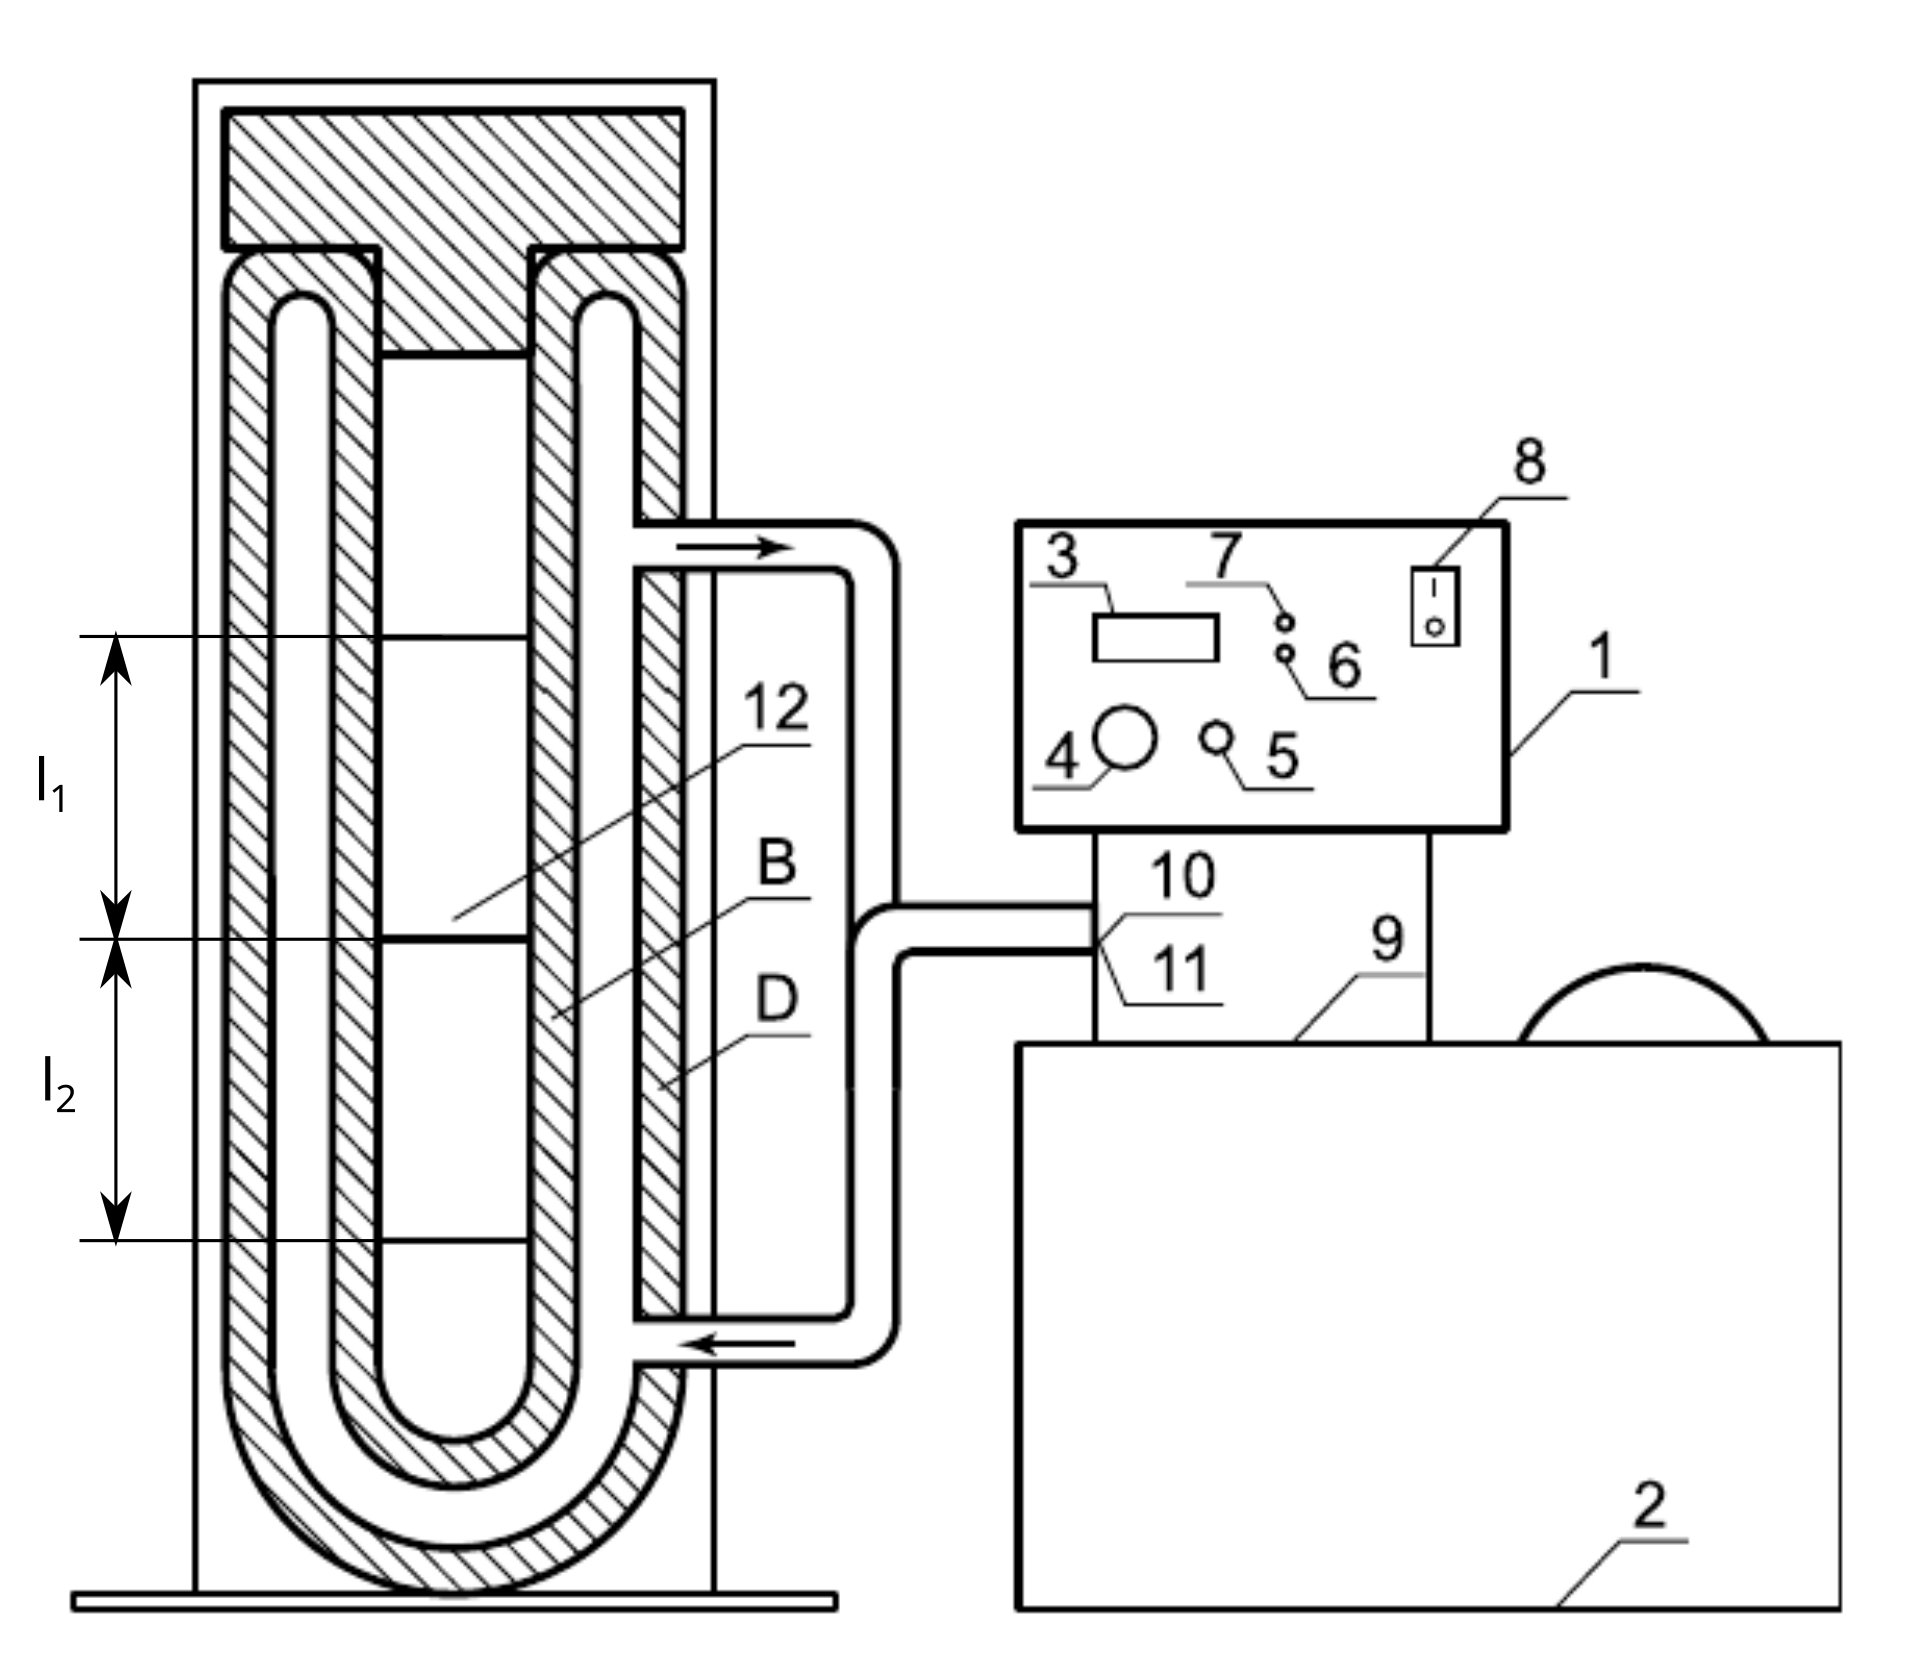
\includegraphics[scale=0.5]{ustanovka}}
        \caption{Установка для определения коэффициента вязкости жидкости.}
        \label{ustanovka}
    \end{figure}

    \section{Ход работы}
    \subsection{Измерение диаметра шариков}

    Выбираем 12 стальных и 12 стеклянных шариков. Из-за неидеальности формы измерения производим в 2 случайных направлениях при помощи микроскопа и усредняем. Данные измерений приведены в таблице~\ref{diameters}. Погрешность измерений $\sigma_d = 0.02~мм$. Плотности шариков:

    \begin{align*}
        \rho_{стекло}&=(2.5 \pm 0.1)~г/см^3\\
        \rho_{сталь}&=(7.8 \pm 0.1)~г/см^3
    \end{align*}

    \begin{table}[!ht]
        \centering
        \subtable{
            \begin{tabular}{|c|c|c|}
            \hline
                № & Материал & Диаметр, мм \\ \hline
                1 & Стекло & 2,07 \\ \hline
                2 & Стекло & 2,08 \\ \hline
                5 & Стекло & 2,11 \\ \hline
                6 & Стекло & 2,10 \\ \hline
                9 & Стекло & 2,09 \\ \hline
                11 & Стекло & 2,12 \\ \hline
                13 & Стекло & 2,09 \\ \hline
                14 & Стекло & 2,12 \\ \hline
                17 & Стекло & 2,09 \\ \hline
                18 & Стекло & 2,12 \\ \hline
                21 & Стекло & 2,12 \\ \hline
                22 & Стекло & 2,16 \\ \hline
            \end{tabular}
        }
        \subtable{
            \begin{tabular}{|c|c|c|}
            \hline
                № & Материал & Диаметр, мм \\ \hline
                3 & Сталь & 0,85 \\ \hline
                4 & Сталь & 0,75 \\ \hline
                7 & Сталь & 0,81 \\ \hline
                8 & Сталь & 0,72 \\ \hline
                10 & Сталь & 0,71 \\ \hline
                12 & Сталь & 0,84 \\ \hline
                15 & Сталь & 0,78 \\ \hline
                16 & Сталь & 0,91 \\ \hline
                19 & Сталь & 0,83 \\ \hline
                20 & Сталь & 0,91 \\ \hline
                23 & Сталь & 0,78 \\ \hline
                24 & Сталь & 0,79 \\ \hline
            \end{tabular}
        }
        \caption{Измеренные диаметры шариков}
        \label{diameters}
    \end{table}

    \subsection{Измерение установившихся скоростей падения шариков}

    Измеренные длины частей цилиндра установки (см. рис.~\ref{ustanovka}):

    \begin{align*}
        l_1 = l_2 = (10.0 \pm 0.1)~см
    \end{align*}

    Измерения производим для 6 значений температуры от 25 до 50 $ ^\circ C $. При помощи секундомера измеряем время прохождения шариком участков $l_1$ и $l_2$ ($ \sigma_t = 2t_{реакц} \approx 0.6~с $). Усредняем значение, вычислеям установившуюся скорость шариков в жидкости. По графику на рис.~\ref{density} определим плотность глицерина для каждой температуры. По формуле~(\ref{eta}) рассчитываем вязкость глицерина ($ \sigma_{\rho_{глиц}} = 0.01~г/см^3 $). Примем $g = (9.81 \pm 0.01)~м/с^2$. Результаты представлены в таблице~\ref{velocities}.

    \begin{figure}[ht]
        \center{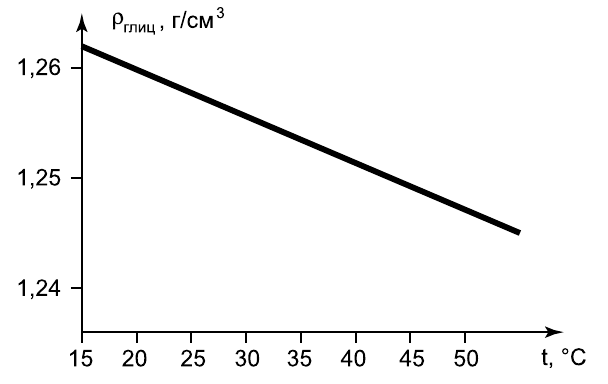
\includegraphics[scale=0.5]{density.png}}
        \caption{График плотности глицерина в зависимости от температуры.}
        \label{density}
    \end{figure}

    \newcolumntype{T}[1]{%
        >{\centering\arraybackslash\hspace{0pt}}p{#1}}%

    \begin{table}[!ht]
        \centering
        \begin{tabular}{|c|c|c|c|c|c|c|T{0.05\textwidth}|T{0.05\textwidth}|T{0.06\textwidth}|T{0.08\textwidth}|T{0.08\textwidth}|}
        \hline
            № & Материал & $T, K$ & $t_{l_1}, с$& $t_{l_2}, с$ & $t_{ср}, с$ & $\sigma{t_{ср}}, с$ & $v_{уст},$ $мм/c$ & $\sigma_{v_{уст}},$ $ мм/c$ & $\rho_{глиц},$ $ г/см^3$ & $\eta,$ $мПа * с$ & $\sigma_{\eta},$ $мПа * с$  \\ \hline
            1 & Стекло & 298 & 27.9 & 27.9 & 27.9 & 0.6 & 3.6 & 0.1 & 1.26 & 809 & 70 \\ \hline
            2 & Стекло & 298 & 27.3 & 27.1 & 27.2 & 0.6 & 3.7 & 0.1 & 1.26 & 796 & 69 \\ \hline
            3 & Сталь & 298 & 29.1 & 29.0 & 29.0 & 0.6 & 3.4 & 0.1 & 1.26 & 748 & 41 \\ \hline
            4 & Сталь & 298 & 34.8 & 34.5 & 34.7 & 0.6 & 2.9 & 0.1 & 1.26 & 695 & 41 \\ \hline
            5 & Стекло & 303 & 18.8 & 18.9 & 18.8 & 0.6 & 5.3 & 0.2 & 1.26 & 568 & 51 \\ \hline
            6 & Стекло & 303 & 18.6 & 18.7 & 18.6 & 0.6 & 5.4 & 0.2 & 1.26 & 557 & 50 \\ \hline
            7 & Сталь & 303 & 21.9 & 21.9 & 21.9 & 0.6 & 4.6 & 0.1 & 1.26 & 512 & 30 \\ \hline
            8 & Сталь & 303 & 26.6 & 26.6 & 26.6 & 0.6 & 3.8 & 0.1 & 1.26 & 492 & 31 \\ \hline
            9 & Стекло & 308 & 12.6 & 12.7 & 12.7 & 0.6 & 7.9 & 0.4 & 1.25 & 376 & 36 \\ \hline
            10 & Сталь & 308 & 17.6 & 18.1 & 17.9 & 0.7 & 5.6 & 0.2 & 1.25 & 322 & 22 \\ \hline
            11 & Стекло & 308 & 12.2 & 12.1 & 12.1 & 0.6 & 8.2 & 0.4 & 1.25 & 371 & 36 \\ \hline
            12 & Сталь & 308 & 14.8 & 15.2 & 15.0 & 0.6 & 6.7 & 0.3 & 1.25 & 378 & 25 \\ \hline
            13 & Стекло & 313 & 8.6 & 8.5 & 8.6 & 0.6 & 11.6 & 0.8 & 1.25 & 255 & 28 \\ \hline
            14 & Стекло & 313 & 8.4 & 8.4 & 8.4 & 0.6 & 11.9 & 0.9 & 1.25 & 257 & 28 \\ \hline
            15 & Сталь & 313 & 10.8 & 11.0 & 10.9 & 0.6 & 9.2 & 0.5 & 1.25 & 237 & 18 \\ \hline
            16 & Сталь & 313 & 8.4 & 8.2 & 8.3 & 0.6 & 12.0 & 0.9 & 1.25 & 246 & 21 \\ \hline
            17 & Стекло & 318 & 6.7 & 6.4 & 6.5 & 0.6 & 15.3 & 1.4 & 1.25 & 195 & 24 \\ \hline
            18 & Стекло & 318 & 6.4 & 6.5 & 6.4 & 0.6 & 15.5 & 1.5 & 1.25 & 198 & 25 \\ \hline
            19 & Сталь & 318 & 8.1 & 8.1 & 8.1 & 0.6 & 12.3 & 0.9 & 1.25 & 199 & 18 \\ \hline
            20 & Сталь & 318 & 7.0 & 6.8 & 6.9 & 0.6 & 14.5 & 1.3 & 1.25 & 204 & 21 \\ \hline
            21 & Стекло & 323 & 4.8 & 4.8 & 4.8 & 0.6 & 20.8 & 2.6 & 1.25 & 148 & 22 \\ \hline
            22 & Стекло & 323 & 4.9 & 4.6 & 4.7 & 0.6 & 21.1 & 2.7 & 1.25 & 151 & 23 \\ \hline
            23 & Сталь & 323 & 5.5 & 5.6 & 5.6 & 0.6 & 18.0 & 2.0 & 1.25 & 121 & 15 \\ \hline
            24 & Сталь & 323 & 5.7 & 5.8 & 5.7 & 0.6 & 17.5 & 1.9 & 1.25 & 127 & 15 \\ \hline
        \end{tabular}
        \caption{Результаты измерений установившившихся скоростей шариков и соответствующих плотностей глицерина}
        \label{velocities}
    \end{table}

    \begin{align*}
        \sigma_{t_{ср}} &= \sqrt{\sigma_t^2 + \sigma_{случ}^2} = \sqrt{\sigma_t^2 + (t - t_{ср})^2}
        & \sigma_{v_{уст}} &= v_{уст}\sqrt{\left( \frac{\sigma_l}{l}\right)^2 + \left(\frac{\sigma_{t_{ср}}}{t_{ср}} \right)^2}\\
         \sigma_{\eta} &= \eta \sqrt{\left( \frac{\sigma_g}{g}\right)^2 + \left( 2\frac{\sigma_d}{d}\right)^2 + \left( \frac{\sigma_{v_{уст}}}{v_{уст}}\right)^2 + \frac{\sigma_{\rho}^2 + \sigma_{\rho_{глиц}}^2}{(\rho - \rho_{глиц})^2}}
    \end{align*}

    Средняя относительная погрешность измерений вязкости $\varepsilon_{\eta} = 9.5\% $

    \subsection{Вычисление числа Рейнольдса, оцена времени и пути релаксации. Анализ применимости формулы Стокса}

    Для каждого из опытов вычислим число Рейнольдса $Re$~(\ref{Re}), оценим время релаксации $\tau$~(\ref{relax_time}) и путь релаксации $S$~(\ref{S}). Результаты представлены в таблице~\ref{re_tau_s}.

    \begin{align}
        Re &= \frac{d}{2} \frac{v_{уст} \rho_{глиц}}{\eta}, & \varepsilon_{Re} &= \sqrt{\left( \frac{\sigma_d}{d} \right)^2 + \left( \frac{\sigma_{v_{уст}}}{v_{уст}} \right)^2 + \left( \frac{\sigma_{\rho_{глиц}}}{\rho_{глиц}} \right)^2 + \left( \frac{\sigma_{\eta}}{\eta} \right)^2}\label{Re}\\
        \tau &= \frac{2}{9} \frac{d^2}{4} \frac{\rho}{\eta}, & \varepsilon_{\tau} &= \sqrt{\left( 2\frac{\sigma_d}{d} \right)^2  + \left( \frac{\sigma_{\rho}}{\rho} \right)^2 + \left( \frac{\sigma_{\eta}}{\eta} \right)^2}\label{relax_time}\\
        S &= v_{уст} \tau, & \varepsilon_S &= \sqrt{\left( \frac{\sigma_{v_{уст}}}{v_{уст}} \right)^2  + \left( \frac{\sigma_{\tau}}{\tau} \right)^2}\label{S}
    \end{align}

    \begin{table}[!ht]
        \centering
        \begin{tabular}{|c|c|c|c|c|c|c|c|c|c|}
            \hline
            № & материал & $T, K$ & $\eta, мПа * с$ & $Re$ & $\sigma_{Re}$ & $\tau, мс$ & $\sigma_{\tau}, мс$ & $S, мкм$ & $\sigma_S, мкм$ \\ \hline
            1 & Стекло & 298 & 809 & 5.8 & 0.5 & 0.74 & 0.07 & 2.64 & 0.06 \\ \hline
            2 & Стекло & 298 & 796 & 6.1 & 0.6 & 0.76 & 0.07 & 2.78 & 0.07 \\ \hline
            3 & Сталь & 298 & 748 & 2.5 & 0.2 & 0.42 & 0.03 & 1.44 & 0.03 \\ \hline
            4 & Сталь & 298 & 695 & 2.0 & 0.1 & 0.35 & 0.03 & 1.01 & 0.02 \\ \hline
            5 & Стекло & 303 & 568 & 12.4 & 1.2 & 1.09 & 0.11 & 5.78 & 0.19 \\ \hline
            6 & Стекло & 303 & 557 & 12.7 & 1.2 & 1.10 & 0.11 & 5.91 & 0.20 \\ \hline
            7 & Сталь & 303 & 512 & 4.5 & 0.3 & 0.56 & 0.04 & 2.54 & 0.07 \\ \hline
            8 & Сталь & 303 & 492 & 3.4 & 0.3 & 0.46 & 0.04 & 1.71 & 0.04 \\ \hline
            9 & Стекло & 308 & 376 & 27.5 & 3.0 & 1.61 & 0.17 & 12.72 & 0.62 \\ \hline
            10 & Сталь & 308 & 322 & 7.7 & 0.7 & 0.68 & 0.06 & 3.79 & 0.14 \\ \hline
            11 & Стекло & 308 & 371 & 29.5 & 3.3 & 1.68 & 0.18 & 13.86 & 0.70 \\ \hline
            12 & Сталь & 308 & 378 & 9.3 & 0.8 & 0.81 & 0.07 & 5.39 & 0.23 \\ \hline
            13 & Стекло & 313 & 255 & 59.7 & 7.8 & 2.38 & 0.28 & 27.69 & 1.96 \\ \hline
            14 & Стекло & 313 & 257 & 61.6 & 8.1 & 2.43 & 0.29 & 28.99 & 2.10 \\ \hline
            15 & Сталь & 313 & 237 & 18.9 & 1.9 & 1.11 & 0.10 & 10.22 & 0.58 \\ \hline
            16 & Сталь & 313 & 246 & 27.9 & 3.2 & 1.46 & 0.14 & 17.56 & 1.29 \\ \hline
            17 & Стекло & 318 & 195 & 102.3 & 16.1 & 3.11 & 0.41 & 47.55 & 4.48 \\ \hline
            18 & Стекло & 318 & 198 & 104.0 & 16.3 & 3.16 & 0.42 & 49.04 & 4.61 \\ \hline
            19 & Сталь & 318 & 199 & 32.1 & 3.9 & 1.50 & 0.15 & 18.50 & 1.38 \\ \hline
            20 & Сталь & 318 & 204 & 40.4 & 5.5 & 1.76 & 0.19 & 25.49 & 2.28 \\ \hline
            21 & Стекло & 323 & 148 & 186.4 & 36.5 & 4.23 & 0.66 & 88.07 & 11.05 \\ \hline
            22 & Стекло & 323 & 151 & 188.4 & 38.0 & 4.29 & 0.69 & 90.69 & 11.79 \\ \hline
            23 & Сталь & 323 & 121 & 72.5 & 12.0 & 2.18 & 0.29 & 39.32 & 4.27 \\ \hline
            24 & Сталь & 323 & 127 & 67.8 & 10.9 & 2.12 & 0.27 & 37.21 & 3.94 \\ \hline
        \end{tabular}
        \caption{Результаты вычисления $Re$, $\tau$, $S$}
        \label{re_tau_s}
    \end{table}

    Итого:

    \begin{align*}
        \langle \varepsilon_{Re} \rangle &= 11.7\%, & \langle \varepsilon_{\tau} \rangle &= 10.8\%, & \langle \varepsilon_S \rangle &= 6.2\%
    \end{align*}

    Как видим, во всех экспериментах число Рейнольдса меньше 1, а путь релаксации пренебрежимо мал. Следовательно формула Стокса применима.

    \subsection{График зависимости $ln \eta$ от $1/T$}

    \begin{figure}[ht]
        \center{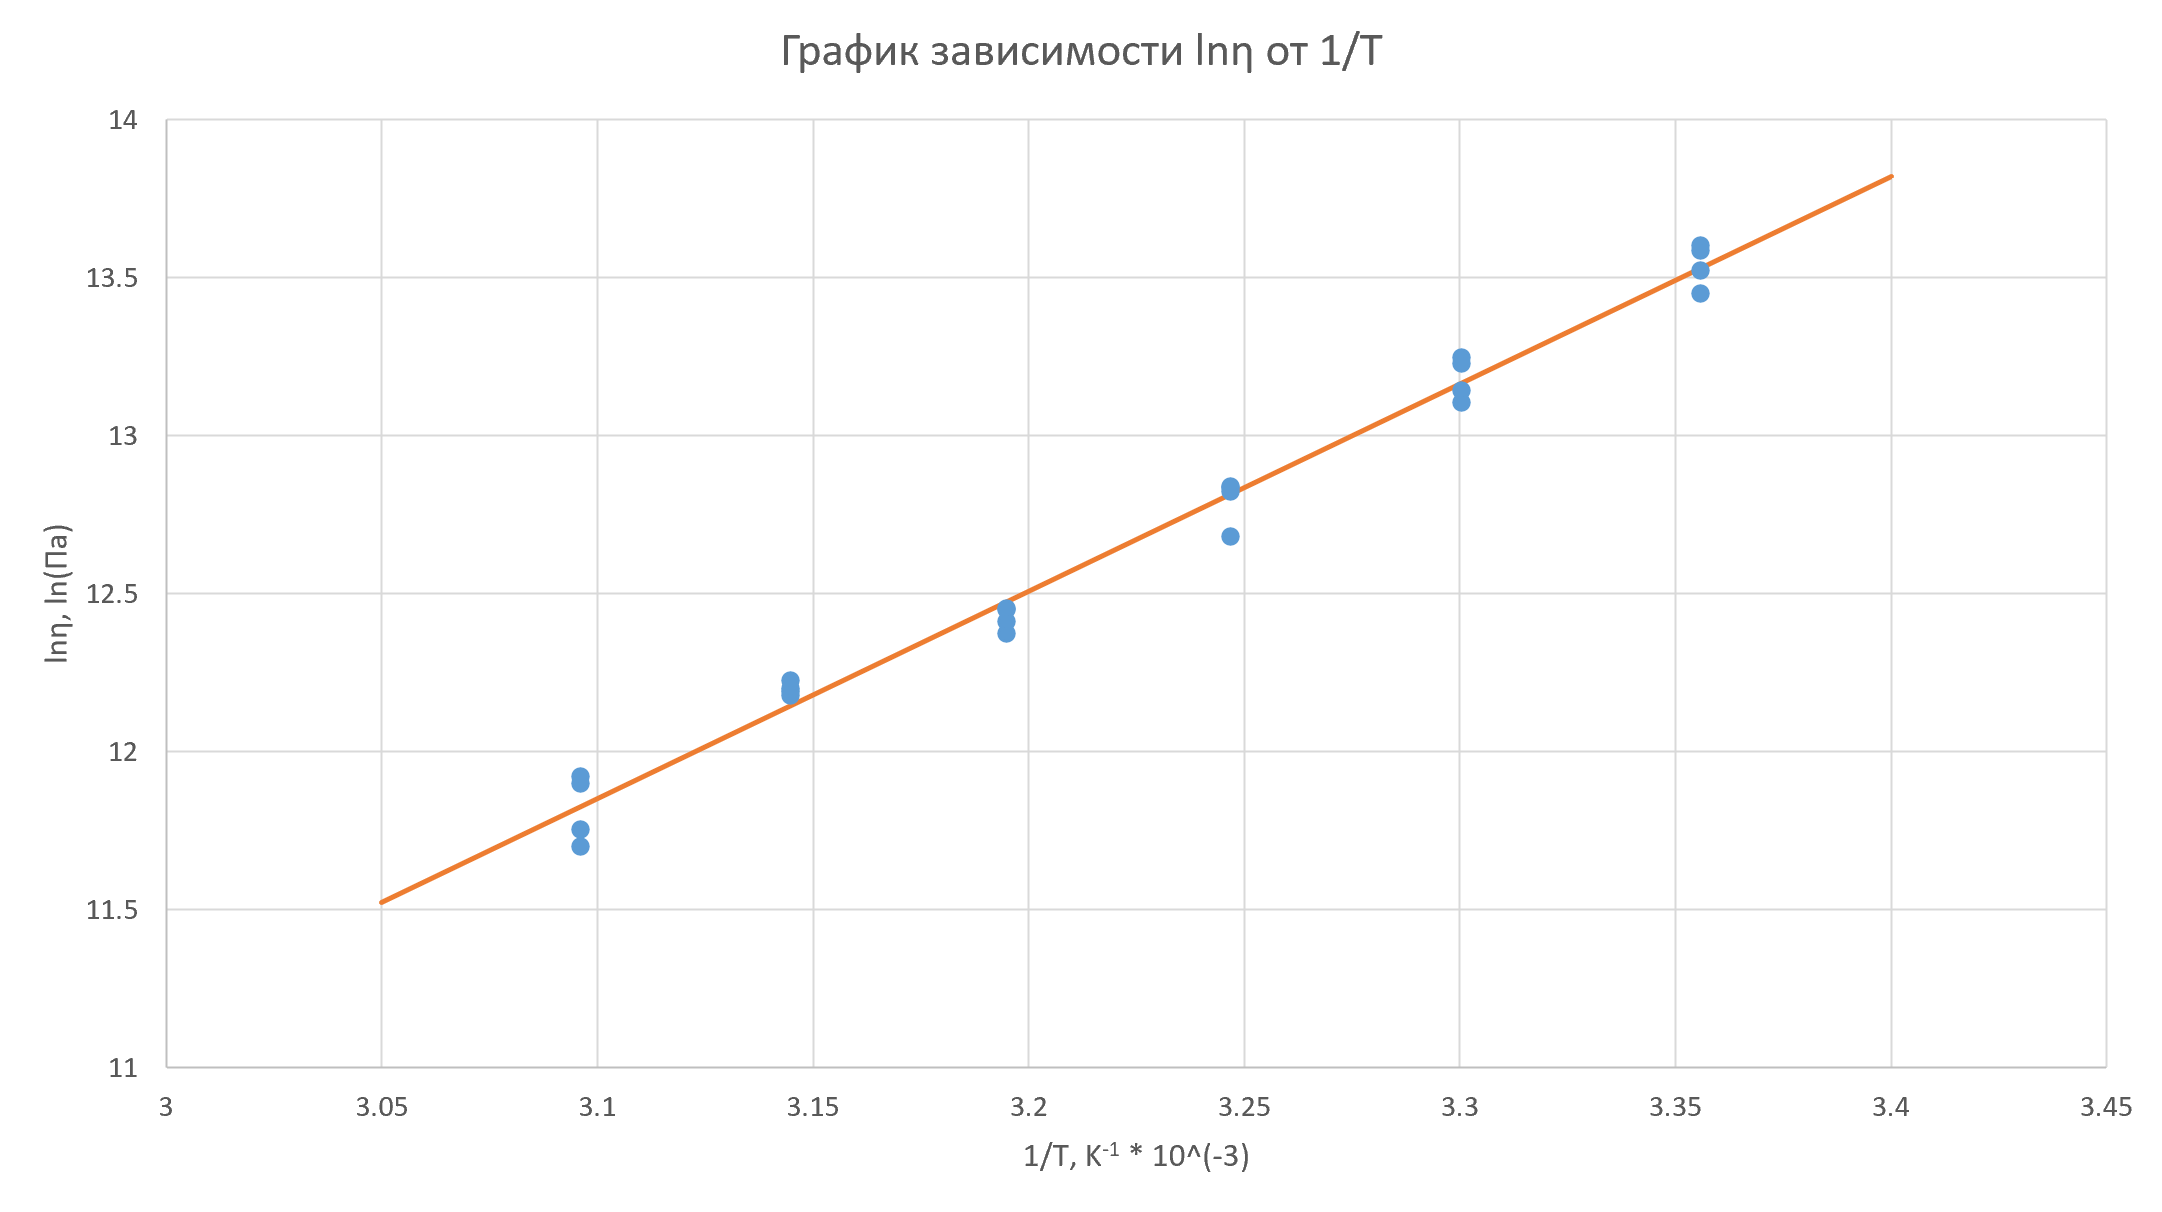
\includegraphics[scale=0.8]{graph.png}}
        \caption{График зависимости $ln \eta$ от $1/T$.}
        \label{graph}
    \end{figure}

    По методу наименьших квадратов вычислим угол наклона прямой.

    \begin{align*}
        k_{накл} = \frac{\langle xy \rangle - \langle x \rangle \langle y \rangle}{\langle x^2 \rangle - \langle x \rangle^2} = (6570 \pm 160) К
    \end{align*}

    Прямая, полученная по МНК не проходит через 0. Это объясняется тем, что в формуле (\ref{activation_energy:1}) есть константа $A$. Коэффициент $b$ прямой соответсвенно равен $lnA$.

    \subsection{Вычисление энергии активации}

    При помощи формулы (\ref{activation_energy:2}) рассчитаем энергию активации:

    \begin{align*}
        W = k * k_{накл} = 1.38 * 10^{-23} Дж/К * 6570~К = 90.7~зДж = 1.511~\frac{кДж}{моль}
    \end{align*}

    \subsection{Оценка погрешностей}

    Случайная погрешность энергии активации:

    \begin{align*}
        \sigma_{k_{накл}} &= \frac{1}{\sqrt{24}} \sqrt{\frac{\langle y^2 \rangle - {\langle y \rangle}^2}{\langle x^2 \rangle - {\langle x \rangle}^2} - k_{накл}^2} = 160~K\\
        \sigma_W^{случ} &= W \frac{\sigma_{k_{накл}}}{k} = 1.511~\frac{кДж}{моль} * 2.4\% = 0.036~\frac{кДж}{моль}
    \end{align*}

    Приборная погрешность энергии активации:

    \begin{align*}
        \sigma_W^{приб} &= W \sqrt{\left( \frac{\sigma_T}{T} \right)^2 + \left( \frac{\sigma_{\eta}}{\eta ln \frac{\eta}{A}} \right)^2} = 0.010~\frac{кДж}{моль}
    \end{align*}

    Полная погрешность энергии активации:

    \begin{align*}
        \sigma_W &= \sqrt{{\sigma_W^{приб}}^2 + {\sigma_W^{случ}}^2} = 0.037~\frac{кДж}{моль}\\
        \varepsilon_W &= 2.5\%
    \end{align*}

    \section{Вывод}

    \begin{align*}
        W = (91 \pm 2)~зДж = (1.51 \pm 0.04)~\frac{кДж}{моль}
    \end{align*}

    Измерили скорости падения шариков при разной температуре жидкости, вычислили вязкость жидкости по закону Стокса и рассчитали энергию активации. Полученная вязкость глицерина при $25^\circ C$ совпадает с табличным значением.

\end{document}
